\paragraph{Test01: GPU vs CPU}
Test configuration:
\begin{itemize}
  \item \textbf{CPU}: Intel(R) Core(TM) i7-4770K CPU @ 3.50GHz 
  \item \textbf{GPU}: NVIDIA Tesla K40c 
\end{itemize}
Implementations tested:
\begin{itemize}
  \item \textbf{legacy\_multifit\_cpu}: plain \textit{cms-sw} cpu code.
  \item \textbf{legacy\_multifit\_gpu}: plain gpu porting \textit{cms-sw} cpu code.
  \item \textbf{multifit\_cpu}: inplace fnnls cpu implementation.
  \item \textbf{multifit\_gpu}: inplace fnnls gpu implementation.
  \item \textbf{multifit\_cpu\_swap}: fnnls cpu implementation with swapping matrices.
  \item \textbf{multifit\_gpu\_swap}: fnnls gpu implementation with swapping matrices.
\end{itemize}
All the cpu implementations are single-threaded. With 64k channels the GPU version achieves a speedup of 2.6. 
\begin{figure}[h]
  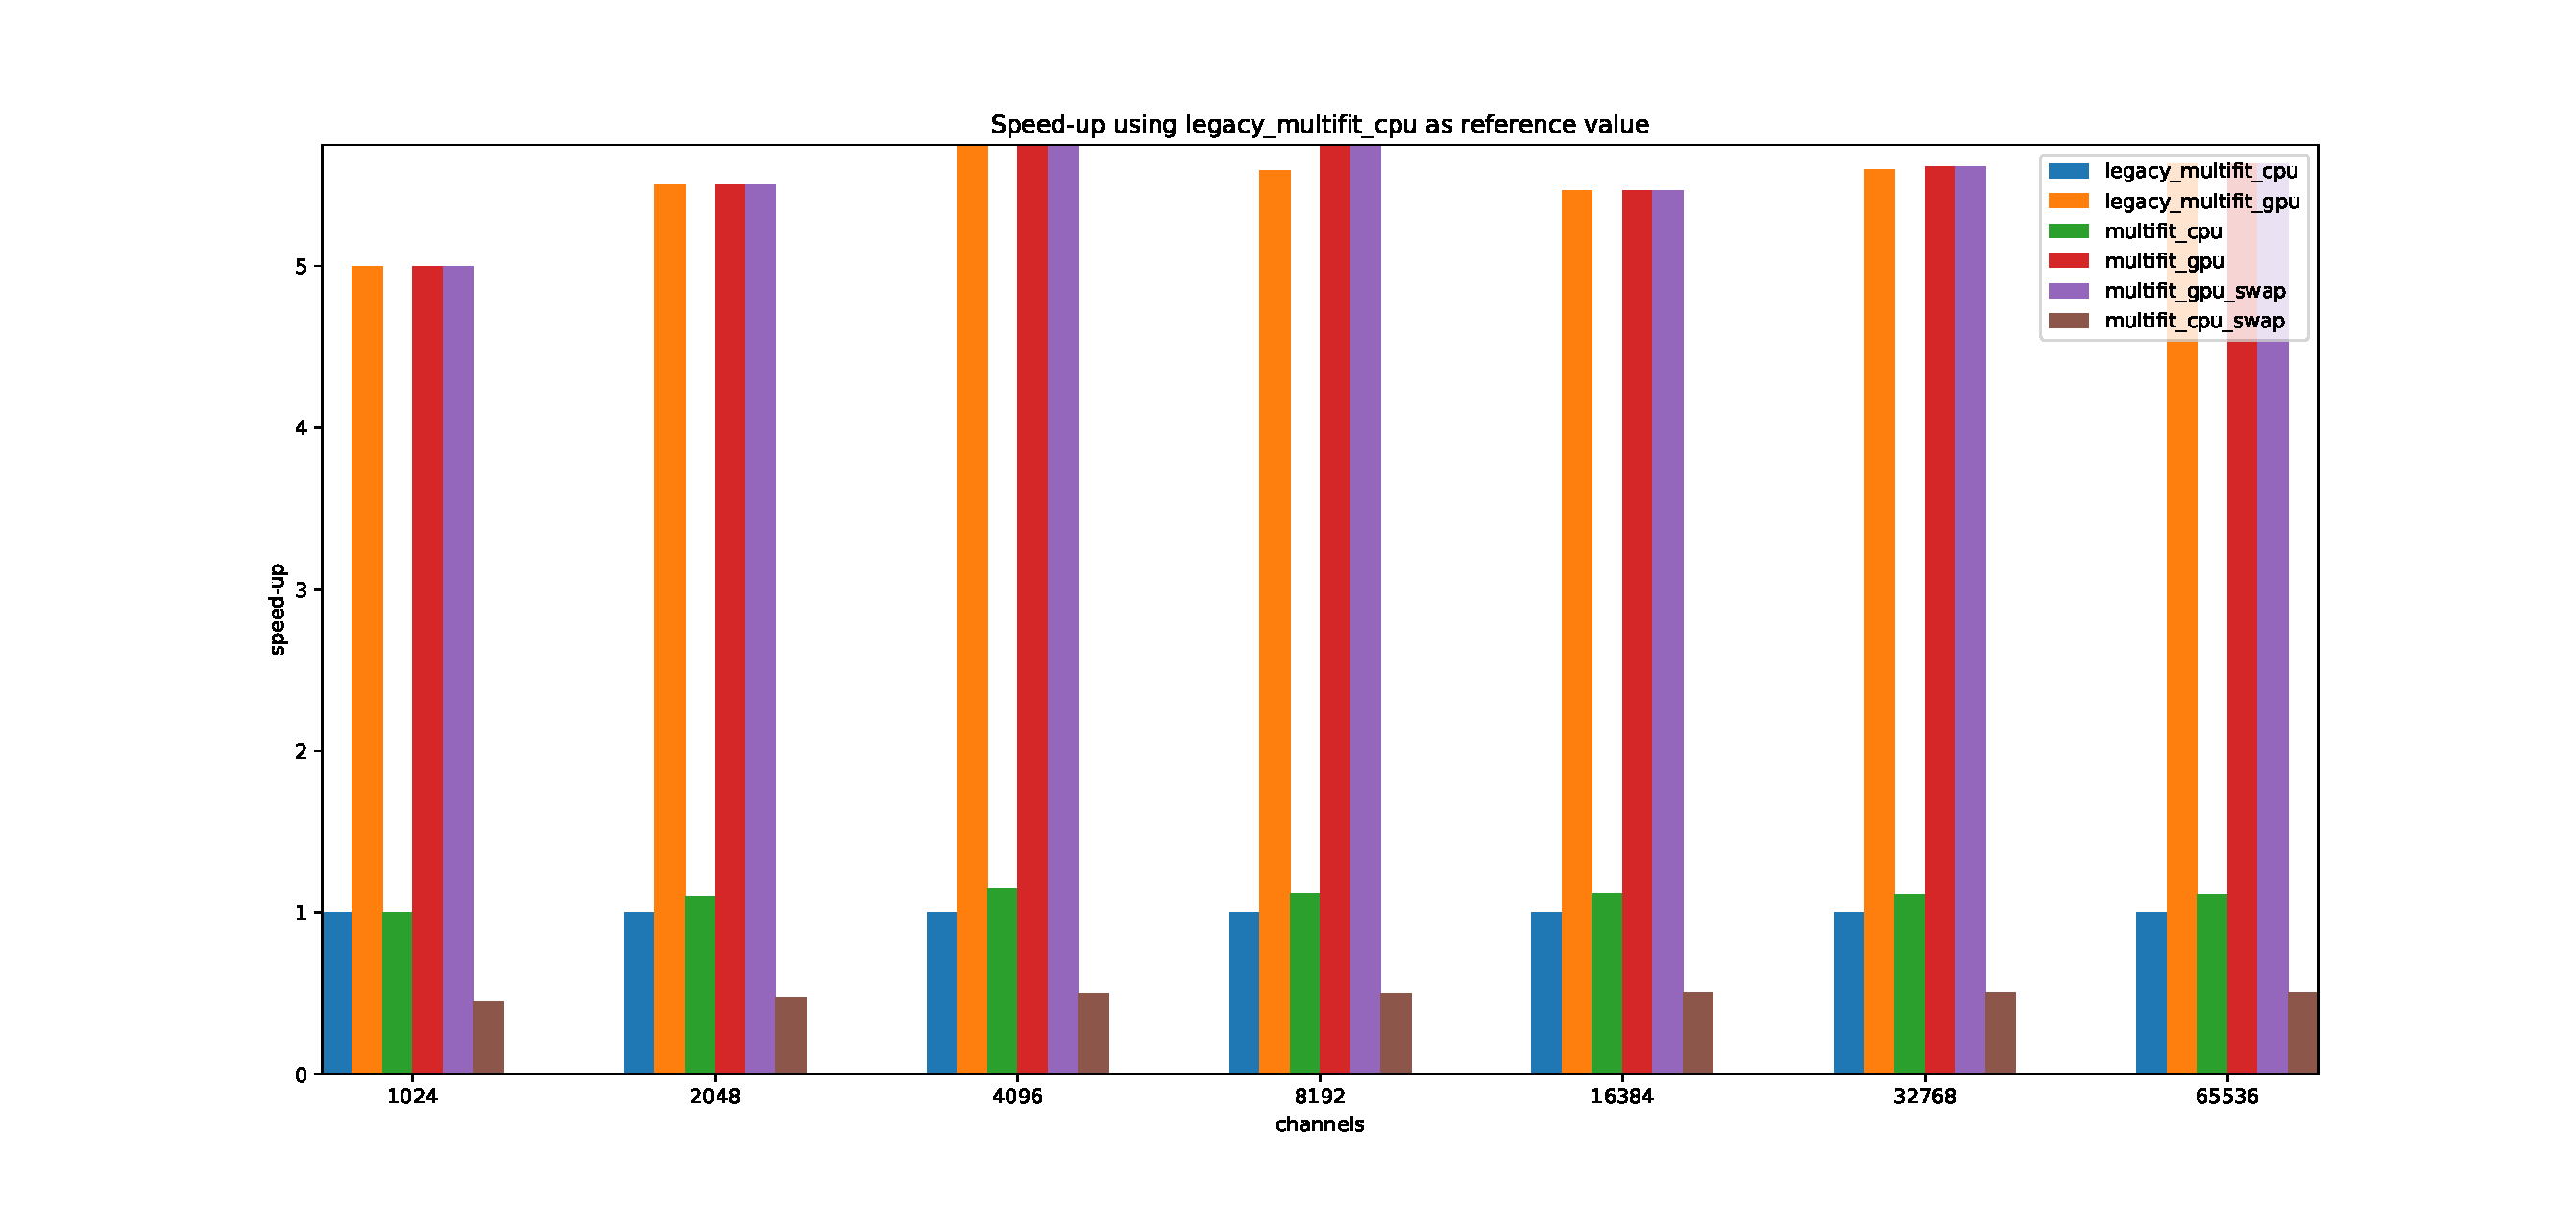
\includegraphics[width=\textwidth]{img/speedup}
  \caption{Speedup achieved with 10 iterations, log channel scale, higher is better}
  \label{img:speedup01}
\end{figure}
\begin{figure}[h]
  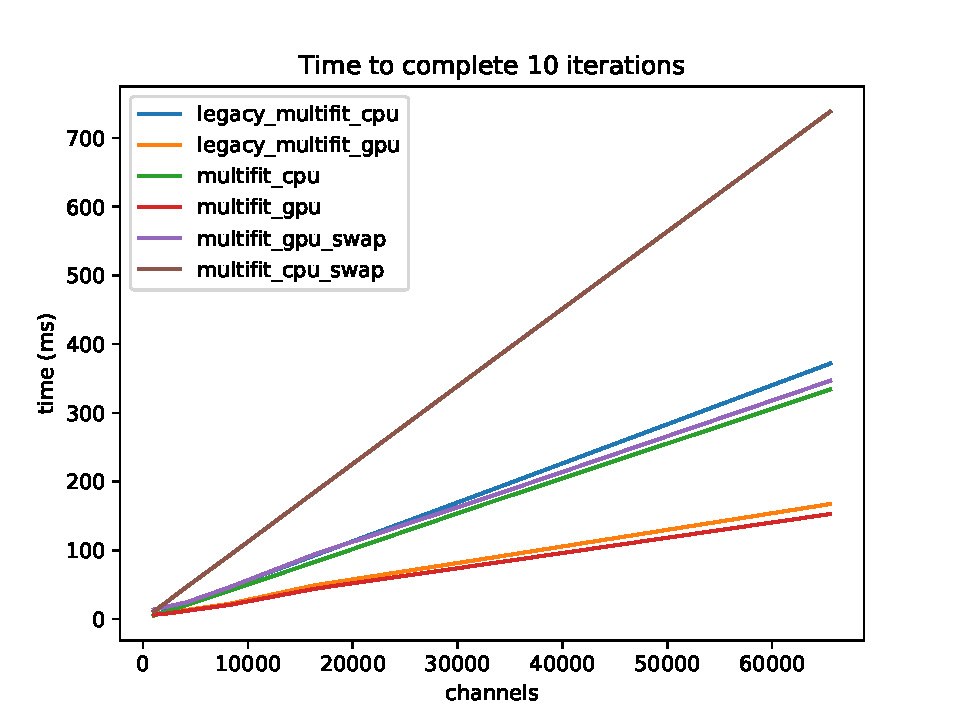
\includegraphics[width=.75\textwidth]{img/linscale}
  \caption{Time needed to complete 10 iterations, linear channel scale, lower is better}
  \label{img:linscale01}
\end{figure}
\begin{figure}[h]
  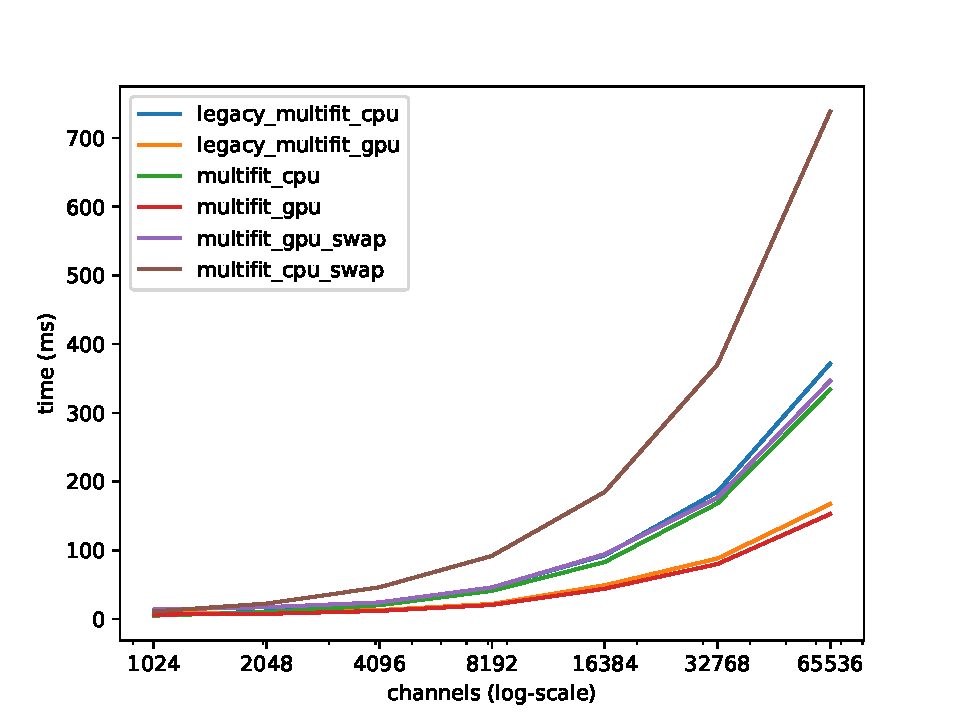
\includegraphics[width=.75\textwidth]{img/logscale}
  \caption{Time needed to complete 10 iterations, log channel scale, lower is better}
  \label{img:logscale01}
\end{figure}

